\chapter{Implementation des BruteForce-Algorithmus}
\label{implementation}
In diesem Kapitel wird die Konzeption des Brute Force-Angriffs beschrieben. Auf Basis der beschriebenen Konzeption wird im Anschluss die Implementation erfolgen. 



\section{Architektur}
In diesem Kapitel wird die geplante Architektur des verteilten Systems beschrieben. \\
Generell wird die Kommunikation nachrichtenbasiert umgesetzt. Dies bedeutet, dass die Komponenten des verteilten Systems kommunizieren, indem sie sich Nachrichten übermitteln können. Die Steuerung der Kommunikation wird primär von den als Master 
(siehe \ref{glossar}) ausgewählten Komponenten umgesetzt. Als Provider wird ein angepasster Webserver eingesetzt, die Verbindung der einzelnen Komponenten zueinander geschieht über WebSockets. Der Webserver basiert auf dem Javascript-Framework Node.js. \\
Details der nachrichtenbasierten Kommunikation werden nun in den folgenden Kapiteln beschrieben. 


\subsection{Nachrichtenstruktur}
Da unsere Implementation auf einer nachrichtenbasierten Kommunikation basieren wird, ist der Entwurf eigener Nachrichtenstrukturen notwendig. Die Nachrichtenstrukturen übertragen alle projektrelevanten Informationen zwischen dem Master und dem Worker oder den Workern. Zur Strukturierung fiel die Wahl auf das Nachrichtenaustauschformat \enquote{JavaScript Object Notation} oder kurz \emph{JSON}, da dieses Format sehr leichtgewichtig und sehr gut anpassbar ist. \\
%TODO WORKER_ID == Hostname/IP
Nachfolgend werden die entwickelten Nachrichtenstrukturen und deren Inhalt detailliert beschrieben. Die Nachrichten werden, je nach Senderichtung, in \emph{Nachrichten zum Worker} und \emph{Nachrichten zum Master} unterteilt. 

\subsubsection{Nachrichten zum Worker}
Hier werden die Strukturen beschrieben, welche vom steuernden Rechner (Master) zu einem der Worker gesendet werden.\\

\texttt{SetupAndConfig}
\begin{lstlisting}[basicstyle=\ttfamily,numbers=left,numberstyle=\footnotesize\ttfamily,backgroundcolor=\color{sourcegray}]
{
  "status" : "setupConfig",
  "value" : {
    "algorithm" : "#HASH_ID",
    "target" : "#TARGET_HASH", 
    "worker_id" : "#WORKER_ID"
  }
}
\end{lstlisting}
Ein im Cluster neu hinzugefügter Worker erhält seine Konfigurationsparameter, damit dieser mit dem Berechnen beginnen kann. 
Der Wert \textbf{algorithm} übergibt die ID des Hash-Algorithmus, welcher in der aktuellen Passwortberechnung benutzt wird. \textbf{Target} übermittelt den Hash des Zielpasswortes. Anhand des Hashes kann ein Worker bestimmen, ob das Zielpasswort berechnet wurde. Die \textbf{workerID} ist eine vom Master vergebene, fortlaufende Nummer und dient der Identifizierung der Worker.\\

\texttt{getWork}
\begin{lstlisting}[basicstyle=\ttfamily,numbers=left,numberstyle=\footnotesize\ttfamily,backgroundcolor=\color{sourcegray}]
{
  "status" : "newWorkBlog",
  "value" : {
    "worker_id" : "#WORKER_ID"
    "hashes" : ["#NEW_HASHES"]
  }
}\end{lstlisting}
Diese Nachricht übermittelt dem Worker eine Anzahl neuer Passwörter, von denen dieser die Hashes berechnen wird.\\
 %TODO Beschreibung fertigstellen.

\texttt{stillAlive}
\begin{lstlisting}[basicstyle=\ttfamily,numbers=left,numberstyle=\footnotesize\ttfamily,backgroundcolor=\color{sourcegray}]
{
  "status" : "stillAlive",
  "value" : ""
}
\end{lstlisting}
Mit Hilfe dieser Nachricht fragt der Master an, ob die angesprochenen Worker noch verfügbar sind. Wenn diese nicht antworten, werden sie aus dem Array der verfügbaren Worker entfernt.


\subsubsection{Nachrichten zum Master}
Folgende Nachrichten werden von den Workern an die Master gesendet. \\

\texttt{newClientRegistration}
\begin{lstlisting}[basicstyle=\ttfamily,numbers=left,numberstyle=\footnotesize\ttfamily,backgroundcolor=\color{sourcegray}]
{
  	"status" : "newClientRegistration",
	"worker" : "#WORKER_ID"
}
\end{lstlisting}
Der Worker beantragt eine ID, um sich im Cluster identifizieren zu können.\\

\texttt{hitTargetHash}
\begin{lstlisting}[basicstyle=\ttfamily,numbers=left,numberstyle=\footnotesize\ttfamily,backgroundcolor=\color{sourcegray}]
{
  "status" : "hitTargetHash",
  "value" : {
    "hash" : "#HASH_VALUE",
    "password" : "#PASSWORD"
    "time_needed" : "#TIME"
    "worker_id" : "#WORKER_ID"
  }
}\end{lstlisting}
Diese Nachricht wird vom Worker versendet, wenn der berechnete Hash dem Zielhash entspricht und somit das Passwort berechnet wurde. Es werden der berechnete Hash und das zugehörige Passwort übertragen. Zudem wird die Zeit, die die Berechnung in Anspruch genommen hat, übertragen. Die Zeit kann für spätere Erweiterungen des Projekts genutzt werden, beispielsweise zum Vergleich verschiedener Hash-Algorithmen.\\
%TODO Beschreibung fertigstellen.

\texttt{finishedWork}
\begin{lstlisting}[basicstyle=\ttfamily,numbers=left,numberstyle=\footnotesize\ttfamily,backgroundcolor=\color{sourcegray}]
{
  "status" : "finishedWork",
  "value" : "#WORKER_ID"
}
\end{lstlisting}
Mit dieser Nachricht teilt der Worker mit, dass alle möglichen Passworte des aktuellen Arbeitspakets berechnet worden sind. Falls bei der Berechnung der Zielhash bzw. das Zielpasswort berechnet worden ist, wird zusätzlich die Nachricht \enquote{finishedWork} versandt. Ansonsten erhält der Worker ein neues Arbeitspaket aus dem Nachrichtenstrom. \\

\texttt{HashesPerTime}
\begin{lstlisting}[basicstyle=\ttfamily,numbers=left,numberstyle=\footnotesize\ttfamily,backgroundcolor=\color{sourcegray}]
{
  "status" : "hashesPerTime"
  "value" : {
    "worker_id" : "#WORKER_ID"
    "hash_count" : "#NUMBER_COMPUTED_HASHES"
    "time_needed" : "#TIME"
  }
}
\end{lstlisting}
Zum Auswerten der ausgeführten Tätigkeiten übermittelt der Worker zur Identifikation seine ID und zur statistischen Auswertung sowohl die Anzahl der berechneten Hashes, als auch die zu dieser Berechnung benötigten Zeit. \\

\texttt{replyAlive}
\begin{lstlisting}[basicstyle=\ttfamily,numbers=left,numberstyle=\footnotesize\ttfamily,backgroundcolor=\color{sourcegray}]
{
  "status" : "alive",
  "value" : "#WORKER_ID"
}
\end{lstlisting}
Der Worker meldet mit dieser Nachricht, dass er dem verteilten System weiterhin zur Verfügung steht. Zur Identifikation antwortet der Worker auf die Nachricht 
\emph{stillAlive} mit seiner Worker-ID. Erfolgt auf die genannte Anfrage keine Antwort, dann entfernt der Master den nicht antwortenden Worker aus dem Array verfügbarer Komponenten.\\

\section{Brute Force-Algorithmus}
\label{ideeBruteForce}
Grundlegend ist das Ziel des Projektes das Entschlüsseln eines vorgegebenen Passwortes. Das zu entschlüsselnde Passwort wird vor der Berechnung vom Benutzer eingetragen. Das eingetragene Passwort wird dann durch eine Hashfunktion geleitet. Der entstandene Hash wird gespeichert und dient als Zielbedingung der folgenden Berechnung. \\
Nun beginnt der eigentliche Angriff. Zu Beginn wird eine sogenannte \enquote{Dictionary-Attack} vorgenommen. Dies bedeutet, dass ein Wörterbuch mit häufig genutzten Passwörtern als Basis des Angriffs genutzt wird. Durch die vorangestellte Attacke auf Basis von häufig benutzten Passwörtern wird die Wahrscheinlichkeit des effizienten Entschlüsseln des gesuchten Passworts erhöht. \\
Bleibt die Dictionary-Attack erfolglos, werden alle möglichen Zeichenkombinationen untersucht. \\
Die erste Idee war es, dass der steuernde Rechner alle möglichen Passwörter in einem Array ablegen wird. Das Muster der möglichen Passwörter sollte wie folgt aufgebaut werden: 

\texttt{Muster der zu berechnenden Passwörter:}
\begin{lstlisting}[basicstyle=\ttfamily,numbers=left,numberstyle=\footnotesize\ttfamily,backgroundcolor=\color{sourcegray}]
	Array passwordsUPPER = 
		[A*****,
	 	B*****,
	 	C*****,
	 	D*****,
	 	...
	]
	
	
	Array passwordsLOWER = 
		[a*****,
	 	b*****,
	 	c*****,
	 	d*****,
		...
	]
	
	

	Array passwordsNUM = 
		[1*****,
	 	2*****,
	 	3*****,
	 	4*****,
		...
	]
\end{lstlisting}

Die exemplarische Darstellung soll die geplante Aufteilung verdeutlichen. Die hier dargestellte feste Länge der Passwörter auf 6 Zeichen dient als Proof Of Concept. Wenn dieses Proof of Concept erfolgreich umgesetzt werden kann, wird in der nächsten Iteration eine variable Passwortlänge ermöglicht. Im ersten Schritt soll die Passwortlänge noch ermittelt werden, bevor die Berechnung der möglichen Passwortkombinationen beginnt. Dadurch wird die Berechnung der Aufgabenverteilung vereinfacht. Wenn auch dieser Meilenstein erfolgreich implementiert werden kann, soll in der nächsten Iteration die Berechnung ohne bekannte Passwortlänge durchgeführt werden. Dies bedeutet implizit, dass die Berechnungsdauer durch die gewachsene Anzahl an möglichen Passwortkombinationen stark ansteigt. Dadurch dann die Robustheit der konzipierten verteilten Architektur geprüft werden. \\

\begin{figure}[!ht]
	\centering
		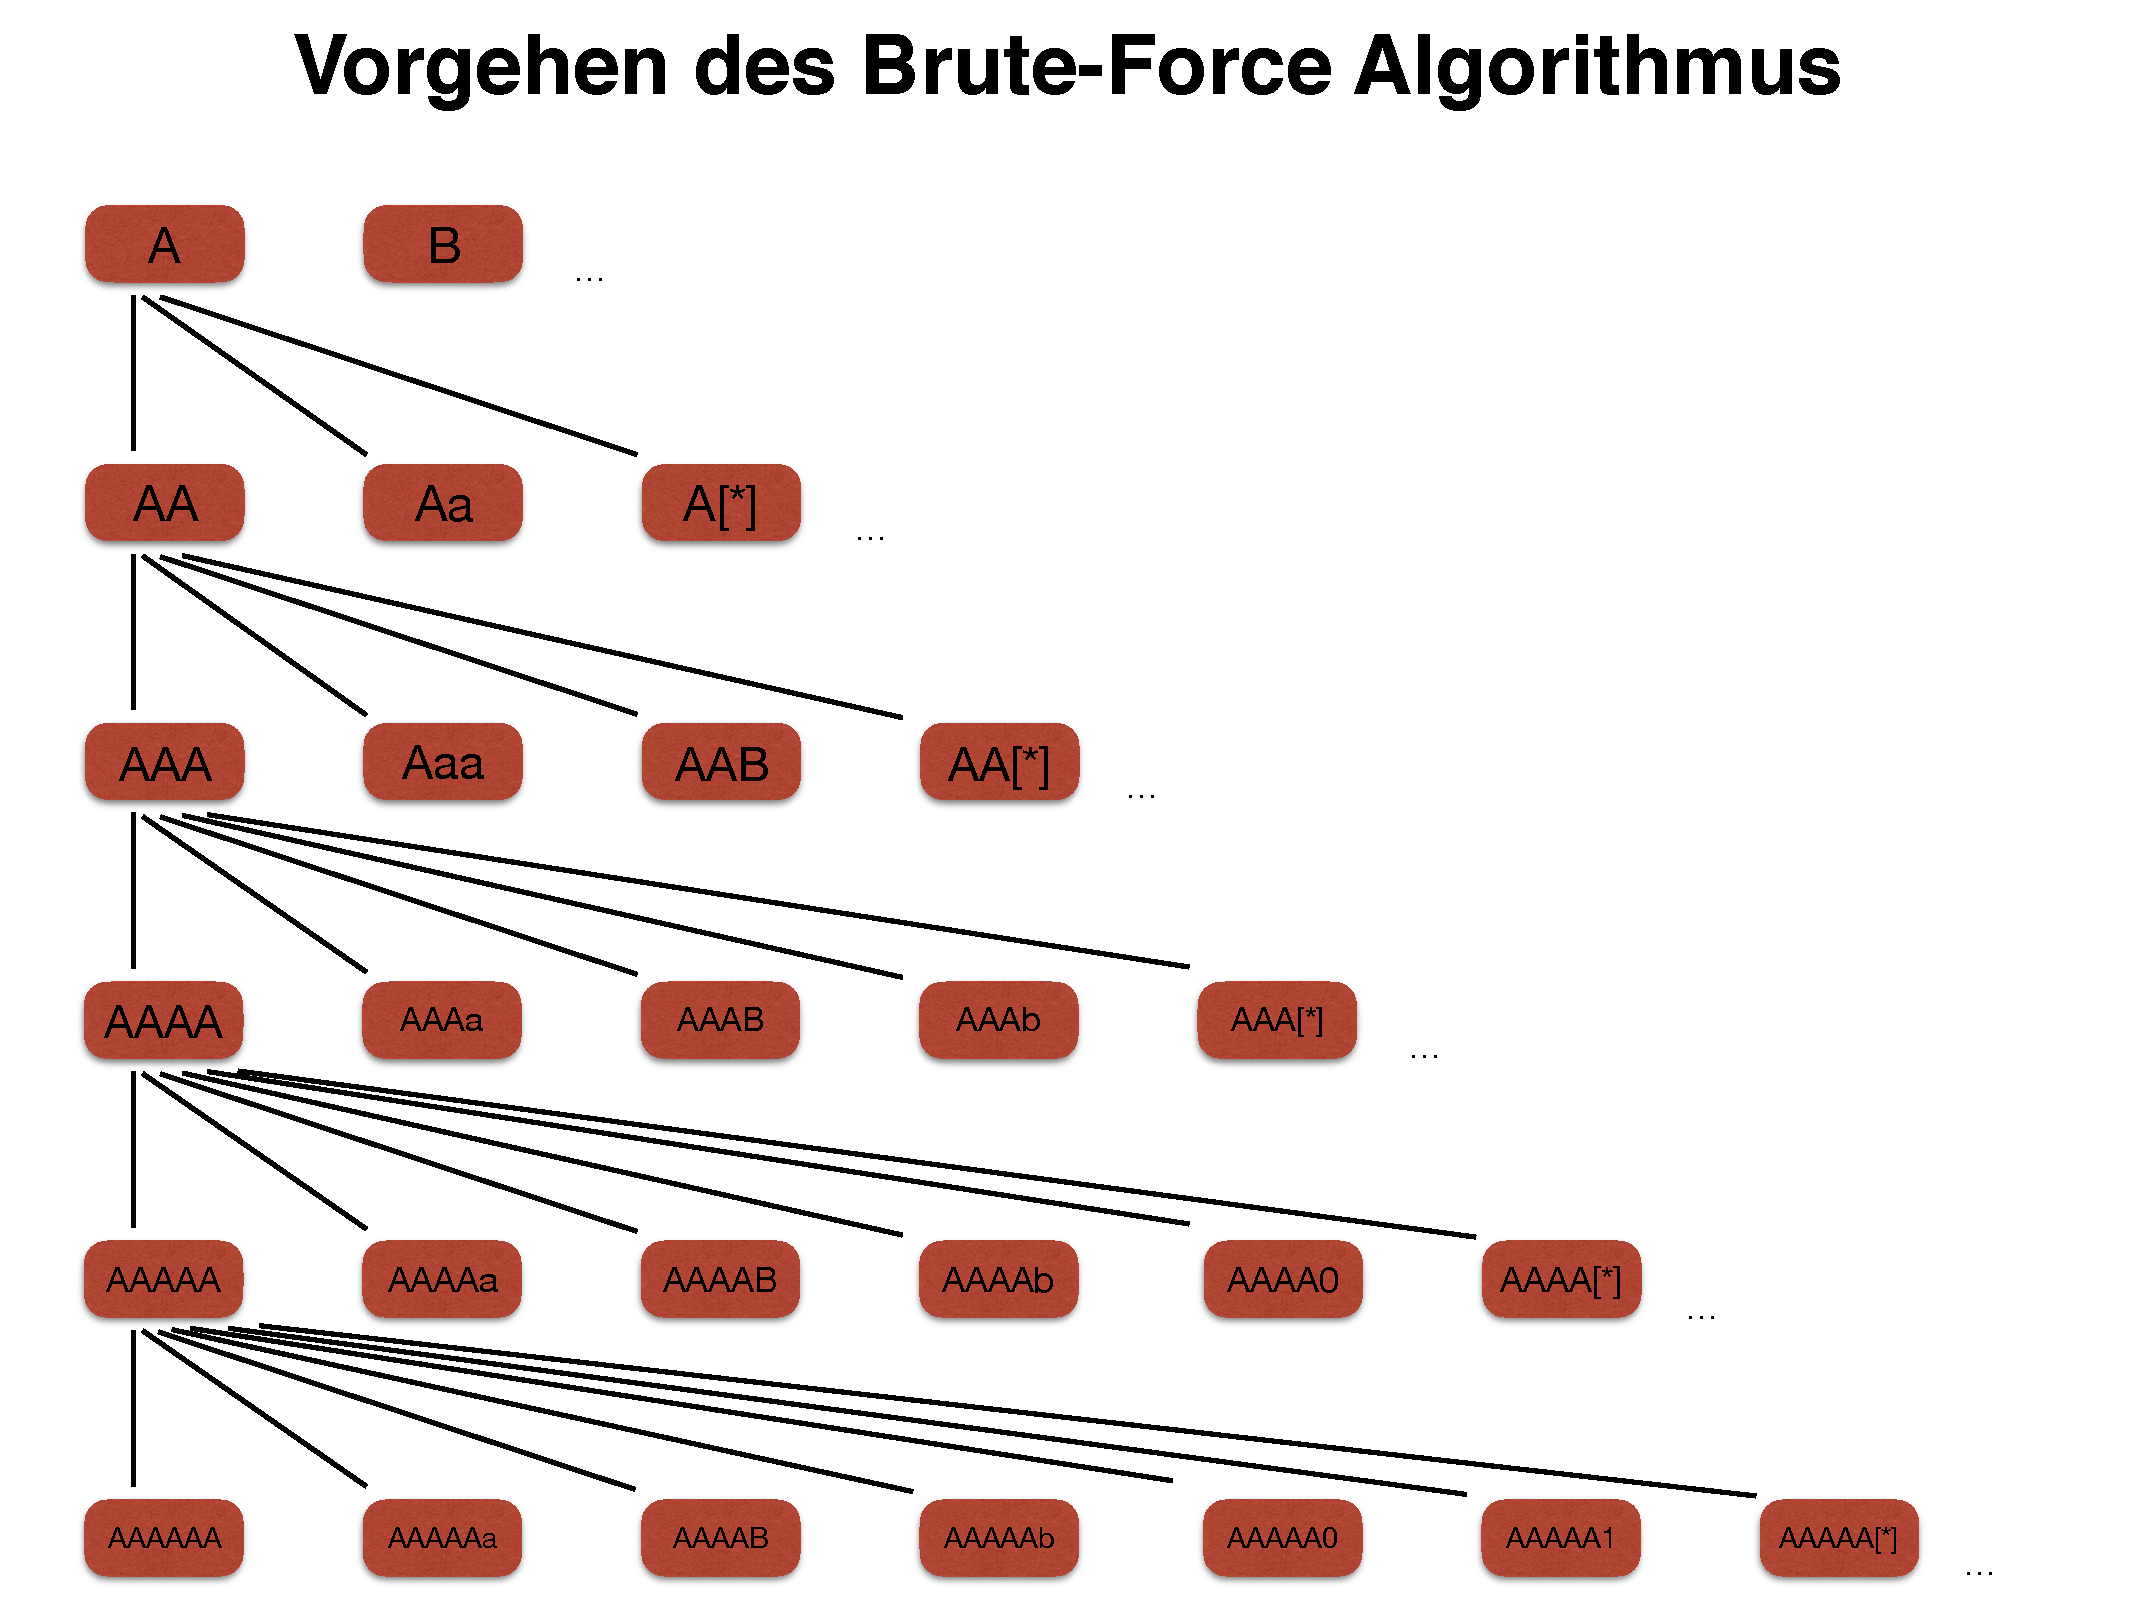
\includegraphics[natwidth=1200pt, natheight=349pt, width=1.0\textwidth]{images/SchaubildAlgorithmBreitensuche.pdf}
	\caption{Darstellung der Suchstrategie, die der Brute-Force Algorithmus zum Ermitteln des Passwortes benutzt.}
	\label{fig:showcase}
\end{figure}

%Hier Breitensuche einfügen

\section{Benutzeroberfläche}

Um Rückschlüsse auf die Geschwindigkeit verschiedener Hash-Algorithmen schließen zu können, kann bei Start der Applikation zwischen verschiedenen Hash-Algorithmen gewählt werden. Zur Auswahl stehen die Hash-Algorithmen \emph{MD5}, \emph{SHA 128} sowie \emph{SHA 256}. Die Geschwindigkeitsunterschiede beruhen primär auf der unterschiedlichen Schlüssellänge der jeweiligen Algorithmen.

\begin{figure}[!ht]
	\centering
		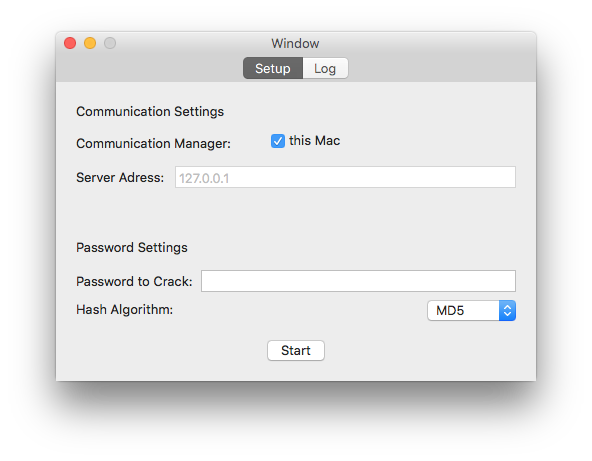
\includegraphics[natwidth=1200pt, natheight=349pt, width=0.6\textwidth]{images/WindowMaster.png}
		\caption{Benutzeroberfläche der implementierten Anwendung als Master der verteilten Anwendung}
	\label{fig:WindowMaster}
\end{figure}



\begin{figure}[!ht]
	\centering
		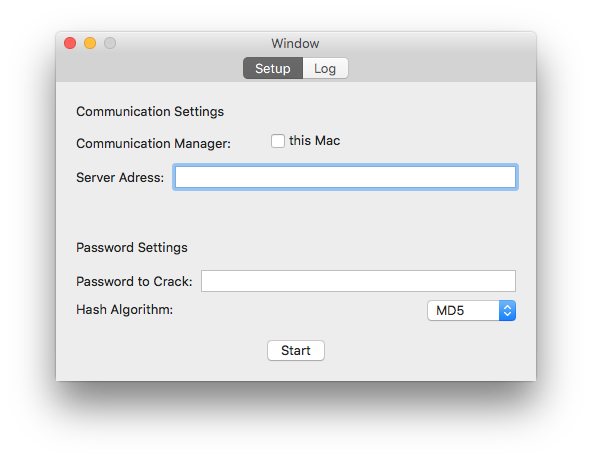
\includegraphics[natwidth=1200pt, natheight=349pt, width=0.6\textwidth]{images/WindowWorker.png}
		\caption{Benutzeroberfläche der implementierten Anwendung als Worker der verteilten Anwendung}
	\label{fig:WindowMaster}
\end{figure}


